\section{Model architecture and training}
This chapter describes the architecture of the neural model used to calculate a similarity score for a given sentence tuple and how this model is trained.

\subsection{Model architecture}
The model consists of a sentence embedding unit and a similarity function. The embedding unit translates a sequence of tokens into a single embedding vector and is applied to the two input sentences using identical weights, thus our system follows a siamese structure \autocite{bromley_signature_1994}. %\textcite{he_multi-perspective_2015}: "Our model has a “Siamese” structure (Bromley et al., 1993) with two subnetworks each processing a sentence in parallel. The subnetworks share all of their weights, and are joined by the similarity measurement layer, then followed by a fully connected layer for similarity score output."
It calculates the sentence embedding by gathering the individual embeddings for the contained tokens, eventually enhancing them with additional information, and applying a composition function. The two resulting embeddings are fed into the similarity function that produces the similarity score. 

Figure~\ref{fig:model_architecture} shows this architecture. In the following, we describe the respective modules. 

\begin{figure}[htb!]
	\centering
	%\textbf{Deviations from gold score}\par\medskip
	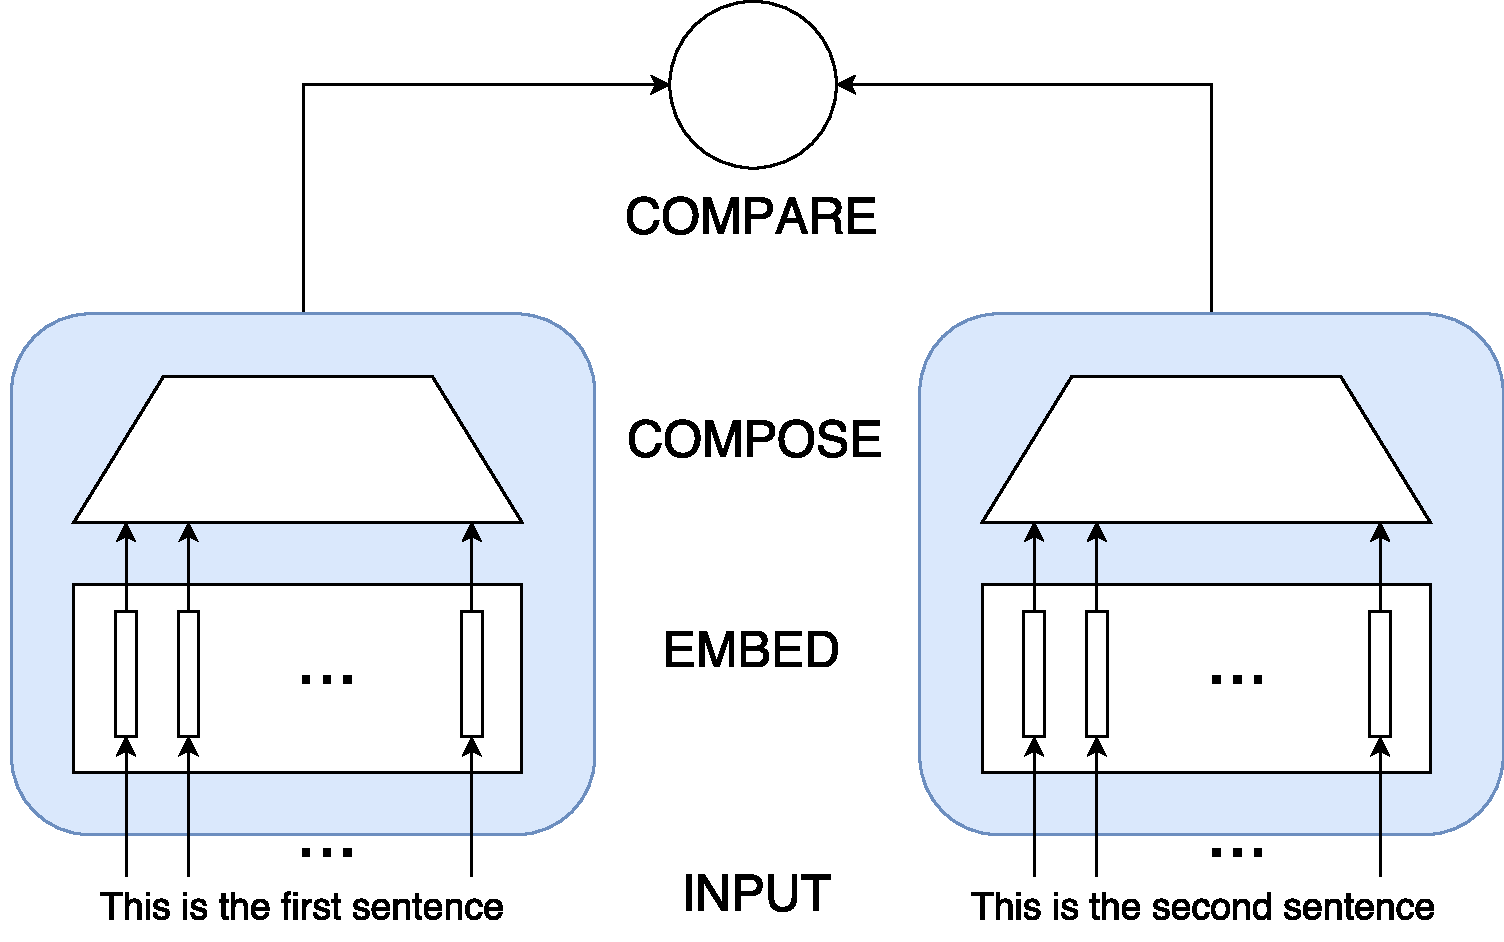
\includegraphics[width=.8\linewidth]{model/SA_model.pdf}
	\caption{General model architecture. The functionality marked by the blue boxes is identical for both input sentences, i.e. they share structure and weights.}
	\label{fig:model_architecture}
\end{figure}

\subsubsection{Token Embeddings}
We use 300 dimensional GloVe vectors \todo{AB:emphasize why glove} \autocite{pennington_glove_2014} to embed individual word tokens. To evaluate the influence of dependency types, we concatenate the embedding with the one-hot encoded dependency type. The dependency type tag set is based on the Universal Dependencies project \autocite{nivre_universal_2016} and includes 40 different types, resulting in 340 dimensional vectors as input for the composition function. When disabling this feature, we set these 40 entries to zero. The embedding weights are not optimized during training.   

\subsubsection{Composition function}
In this work, we compare two major settings: Using (1) \acf{AVG} or (2) \acf{LSTM} as composition function. 
In the \ac{AVG} case, we apply one \acf{FC} with $tanh$ as activation function to every token embedding. Then, averaging the resulting vectors gives the sentence embedding.
In the \ac{LSTM} setting, the token embeddings are fed directly into a LSTM layer whose final state output is used as sentence embedding. %The two settings are visualized in Figure~\todo{AB: add figure}.

To achieve comparability between the two composition functions, we control the amount of effectively trainable parameters in each of them. Depending on whether dependency parse information is used, we use different sizes for the $tanh$ \ac{FC} in the \ac{AVG} case and the inner state of the \ac{LSTM} to fix the amount of effective parameters to approximately 111000. Table~\ref{tab:sizes} shows the exact amounts and sizes of the elements. % total sizes: AVG=input*fc, LSTM=(input+state+1)*4*state 

\begin{table}[!htb]
  \centering
  \begin{tabular}{ l | c | c }
      & AVG (FC size) & LSTM (state size) \\ \hline
    w/ dependency edge & 110840 (326) & 111248 (68) \\ 
    w/o dependency edge & 111000 (370) & 111000 (74) \\
  \end{tabular}
  \caption{Amounts of trainable parameters and sizes of composition function elements}
  \label{tab:sizes}
\end{table}

\subsubsection{Similarity calculation}
We use the cosine similarity to calculate the similarity score between the two sentence embeddings as described in section~\ref{subsec:similarity_measure}:
\begin{equation}
f_{SIM_{cos}}(a,b) = \frac{a \cdot b}{\norm{a}_2\norm{b}_2} 
\end{equation}

\subsubsection{Baseline model}
As baseline of comparison we calculated TF-IDF based similarity scores in the following manner. We parse and lemmatize each sentence and filter for verbs, nouns and adjectives according to POS tags. Then, we embed each sentence with TF-IDF as described in section~\ref{subsec:doc_embedding} and apply the similarity measure as usual. 

\subsection{Training and Implementation}
We train the model via batched back-propagation with the \ac{MSE} loss function described in section~\ref{subsec:cost_function} and apply ADAM \autocite{kingma_adam_2014} %ADADELTA \autocite{zeiler_adadelta_2012}
as optimizer. We use a 4:1 train/dev split for early stopping. The training is terminated when the score on the development data set does not increase anymore regarding a smoothing window covering the last 25 epochs. 

The model is implemented with the TensorFlow framework  \autocite{abadi_tensorflow_2016}. TensorFlow allows to define and to execute arbitrary dataflow graphs efficiently on different devices as CPUs or GPUs. For tokenization and dependency parsing we use spaCy\footnote{see \url{https://spacy.io/}} which is a fast and still accurate\footnote{see \textcite{choi_it_2015} for a comparative study} \ac{NLP} framework. 


%\subsection{Pre-Training}
%To increase the amount of available training examples, we examined pre-training on a dataset that is one order of magnitude larger than the SICK corpus. We train the models on this data until the early stopping criterion is met and use the resulting weights to initialize the models trained on the SICK dataset. 




